\documentclass{beamer}
\usepackage{amsmath, amssymb}
\usepackage{graphicx}
\usepackage{listings}
\usepackage{color}
\usepackage{subfig}
\usepackage{hyperref}
\usepackage{tcolorbox,fancyvrb,xcolor,tikz}
\tcbuselibrary{skins,breakable}

\newenvironment{VerbatimIN}
 {\VerbatimEnvironment
  \begin{tcolorbox}[
    breakable,
    colback=lightgray,
    spartan
  ]%
  \begin{Verbatim}}
 {\end{Verbatim}\end{tcolorbox}}

 \newenvironment{VerbatimOUT}
 {\VerbatimEnvironment
  \begin{tcolorbox}[
    breakable,
    spartan
  ]%
  \begin{Verbatim}}
 {\end{Verbatim}\end{tcolorbox}}



\title{Mixed Effects Models - Day 7}
\subtitle{Diagnostics of Mixed Effects Models}
\author{Marieke Wesselkamp\\Department of Biometry and Environmental Systems Analysis\\Albert-Ludwigs-University of Freiburg (Germany)}
\date{February 2023}

\begin{document}

\frame{\titlepage}

\begin{frame}
    \frametitle{The Linear Mixed Effects Model}
    \[
    \mathbf{y} = \mathbf{X} \cdot \mathbf{b} + \mathbf{Z} \cdot \mathbf{u} + \mathbf{e}
    \]
    \[
    \mathbf{e} \sim \mathcal{N}(0, \mathbf{R}), \quad \mathbf{u} \sim \mathcal{N}(0, \mathbf{G}), \quad \mathbf{u} \bot \mathbf{e}
    \]
    where:
    \begin{itemize}
        \item $\mathbf{y}$: measured response values
        \item $\mathbf{X}$: Fixed Effects design matrix
        \item $\mathbf{b}$: Fixed Effects parameter vector of $\mathbf{X}$
        \item $\mathbf{e}$: Vector of the errors $\epsilon$, which are normally distributed (mean = 0; variance by residual variance-covariance matrix \textbf{R})
    \end{itemize}
\end{frame}

\begin{frame}
    \frametitle{Stochastic Components of Mixed Effects Models}
    \begin{itemize}
        \item The \textbf{first stochastic part} describes how random effects parameters $\mathbf{u}$ vary around 0 and is given by the random effects variance-covariance matrix \textbf{G}
        \[
        \mathbf{u} \sim \mathcal{N}(0, \mathbf{G})
        \]
        \item The \textbf{second stochastic part} describes the remaining and unexplained (\textit{residual}) variance:
        \[
        \mathbf{e} \sim \mathcal{N}(0, \mathbf{R})
        \]
        It describes how the measurements \textbf{e} vary around 0, \textbf{After} accounting for the fixed and random effects and is given by the residual variance-covariance matrix \textbf{R}.
    \end{itemize}
\end{frame}

\begin{frame}
    \frametitle{Assumptions of Mixed Effects Models}
    \begin{enumerate}
        \item $\mathbf{b}$ describes the deterministic trend averaged over the random effects $\mathbf{u}$.
        \item Random effects $\mathbf{u}$ are normally and independently distributed among groups with $\mathit{mean = 0}$ and covariance matrix $\mathbf{G}$.
        \item Residual errors $\mathbf{e}$ are normally and independently distributed within a group with $\mathit{mean = 0}$ and variance $\sigma^2$.
        \item $\mathbf{u}$ and $\mathbf{e}$ are independent of each other: among groups, there are no correlation of errors 
        \item Variances and covariances do not depend on group: they are homogeneous, each group has the same values.
    \end{enumerate}
\end{frame}

\begin{frame}
    \frametitle{Assumptions of Mixed Effects Models}
    \begin{enumerate}
        \item $\mathbf{b}$ describes the deterministic trend averaged over the random effects $\mathbf{u}$.
        \item Random effects $\mathbf{u}$ are normally and independently distributed among groups with $\mathit{mean = 0}$ and covariance matrix $\mathbf{G}$.
        \item Residual errors $\mathbf{e}$ are normally and independently distributed within a group with $\mathit{mean = 0}$ and variance $\sigma^2$.
        \item $\mathbf{u}$ and $\mathbf{e}$ are independent of each other: among groups, there are no correlation of errors 
        \item Variances and covariances do not depend on group: they are homogeneous, each group has the same values.
    \end{enumerate}
    \vspace{0.2cm}
    
    \textbf{Violations of these assumptions can lead to problems with residuals and fitting. Each assumption must be tested.}
\end{frame}

\begin{frame}
    \frametitle{Model Specification: Key Components}
    \textbf{The key to a well behaved model is to specify your model correctly. For MEMs there are three parts to be specified:}
    \vspace{0.2cm}
    
    \begin{itemize}
        \item The fixed (deterministic) effects part
        \item The random effects part
        \item The residual variance part
    \end{itemize}
\end{frame}

\begin{frame}
    \frametitle{The recipe to a good model}
    \begin{itemize}
        \item[] \textbf{True for all models:}
        \item define the deterministic part of the model, i.e. find the fixed effects incl. their interactions and potential quadratic / cubic etc. terms.
        \item choose a distribution for the errors
        \item[] 
        \item[] \textbf{Additionally for Mixed Effect Models:}
        \item spot the grouping in the data
        \item how many random effects are there in the data?
        \item if two or more, are they nested or crossed?
        \item can you specify random slopes / random contrasts for one or all of the random effects?
    \end{itemize}
\end{frame}

\begin{frame}[fragile]
    \frametitle{}
    \textbf{The idea of a \color{blue}{sick}} \textbf{model also applies to Mixed Effect Models}
    \vspace{0.2cm}
    \begin{center}
        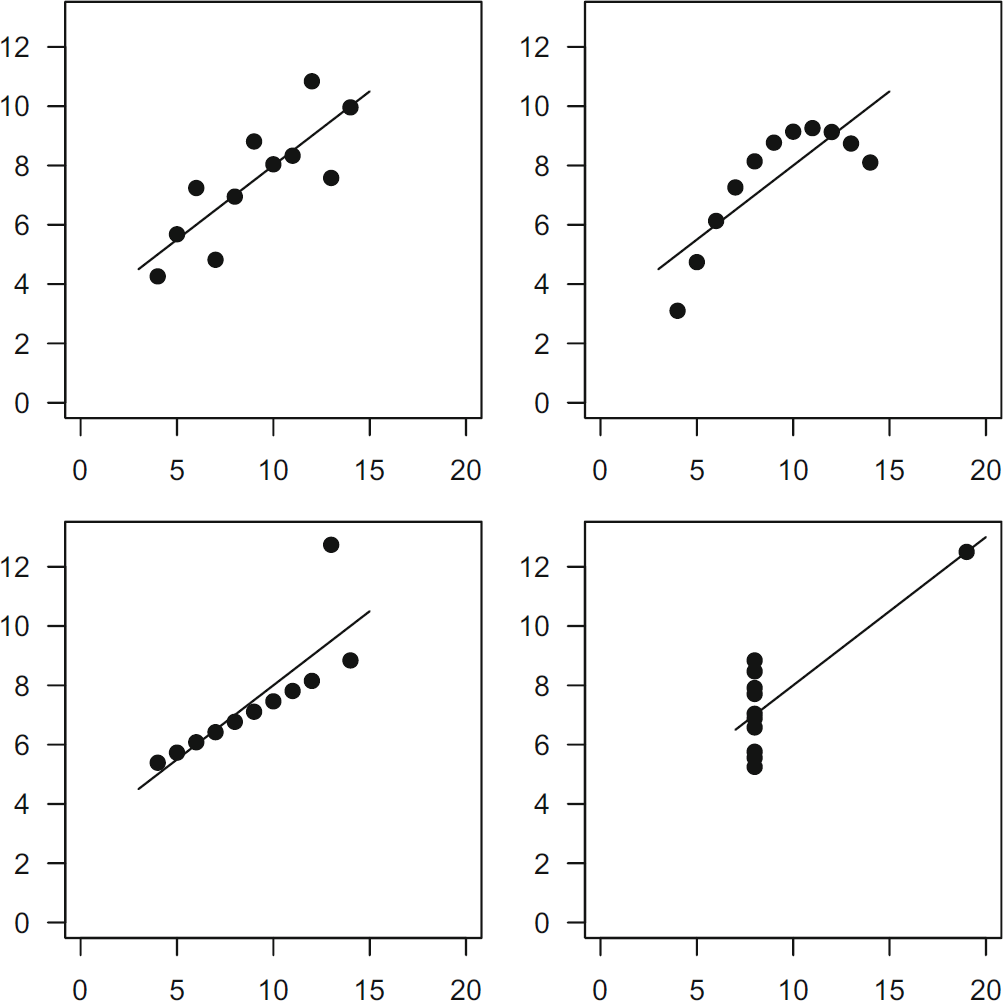
\includegraphics[width=0.6\textwidth]{lectures/day_7_diagnostics_of_mems/figures/Anscombe.png}
    \end{center}
\end{frame}

\begin{frame}
    \frametitle{Residual Checks for LMEMs}
    \begin{center}
    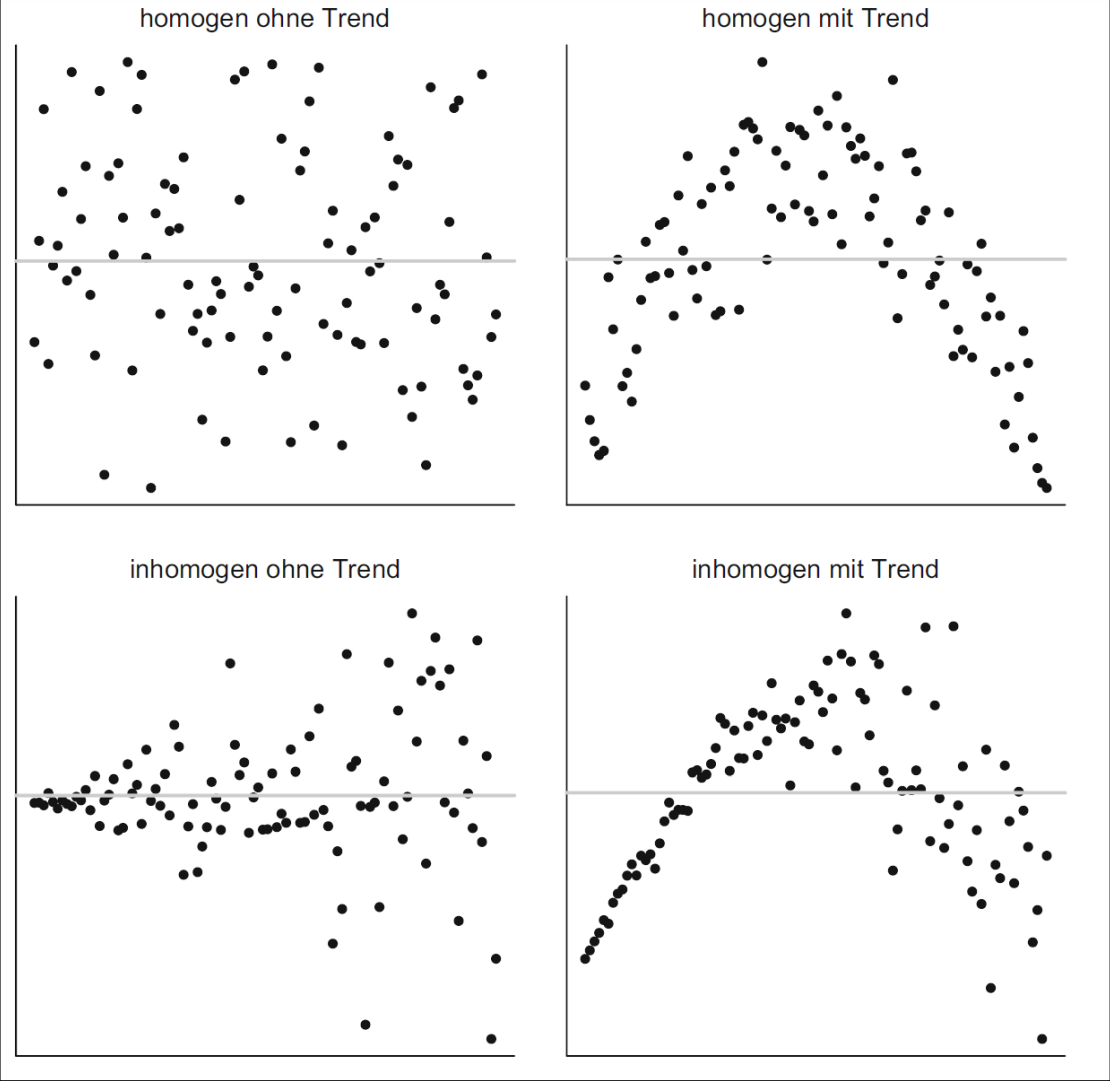
\includegraphics[width=0.6\textwidth]{lectures/day_7_diagnostics_of_mems/figures/residuals.png}    
    \end{center}
    \textbf{Linear Mixed Effects Models (LMEMs) require more checks because they have more assumptions!}
\end{frame}

\begin{frame}
    \frametitle{}
    \huge\color{purple}\textbf{1. Check the Grouping in the Output}
    \vspace{0.5cm}
    
    \normalsize\color{black}\textbf{Example: Glycogen concentration measurements from a nested design involving rats, livers, and preparation methods.}
\end{frame}

\begin{frame}[fragile]
    \frametitle{}
    \begin{columns}
        \begin{column}{0.5\textwidth}
            In 3 treatments the liver of 2 rats each were cut into 3 pieces and per liver piece 2 preparations for glycogen concentration were obtained\\
            = 3 x 2 x 3 x 2 = 36
        \end{column}
        \begin{column}{0.5\textwidth}
            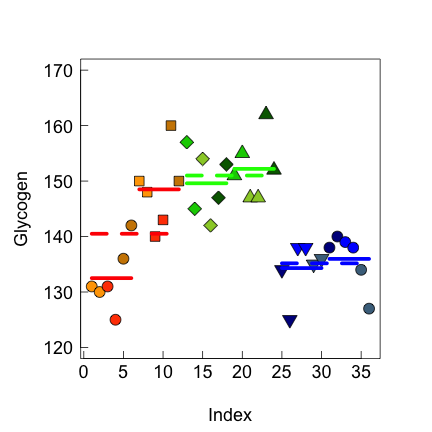
\includegraphics[width=\textwidth]{lectures/day_7_diagnostics_of_mems/figures/unnamed-chunk-3-1.png}
        \end{column}
    \end{columns}
\end{frame}

\begin{frame}[fragile]
    \frametitle{Nested Design}
    \begin{columns}
        \begin{column}{0.6\textwidth}
        \tiny
        \begin{VerbatimIN}
m.r <- lmer(Glycogen~Treatment+(1|Rat/Liver), rats)            
        \end{VerbatimIN}
        \begin{VerbatimOUT}
Linear mixed model fit by REML ['lmerMod']
Formula: Glycogen ~ Treatment + (1|Rat/Liver)
   Data: rats

REML criterion at convergence: 227.1

Scaled residuals: 
     Min       1Q   Median       3Q      Max 
-1.91171 -0.71277 -0.03182  0.71589  2.52546 

Random effects:
 Groups    Name        Variance  Std.Dev. 
 Liver:Rat (Intercept) 1.146e-07 0.0003385
 Rat       (Intercept) 2.061e+01 4.5395756
 Residual              4.248e+01 6.5173452
Number of obs: 36, groups:  Liver:Rat, 6; Rat, 2

Fixed effects:
            Estimate Std. Error t value
(Intercept)  140.500      3.721  37.762
Treatment2    10.500      2.661   3.946
Treatment3    -5.333      2.661  -2.004
optimizer (nloptwrap) convergence code: 0 (OK)
boundary (singular) fit: see ?isSingular            
        \end{VerbatimOUT}
        \end{column}
        \begin{column}{0.4\textwidth}
            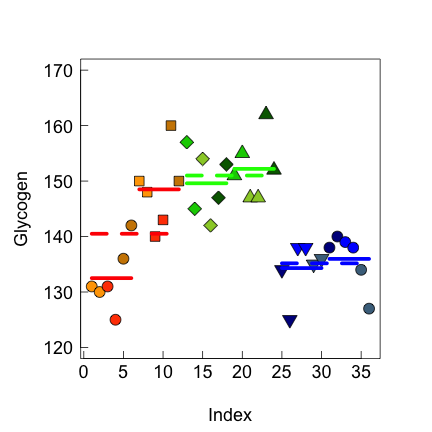
\includegraphics[width=\textwidth]{lectures/day_7_diagnostics_of_mems/figures/unnamed-chunk-3-1.png}
        \end{column}
    \end{columns}
\end{frame}

\begin{frame}[fragile]
    \frametitle{Wrongly Crossed Design}
    \begin{columns}
        \begin{column}{0.6\textwidth}
            \tiny
            \begin{VerbatimIN}
m.r.2 <- 
lmer(Glycogen~Treatment + (1|Rat) + (1|Liver), rats)                
            \end{VerbatimIN}
            \begin{VerbatimOUT}
Linear mixed model fit by REML ['lmerMod']
Formula: Glycogen ~ Treatment + (1|Rat) + (1|Liver)
   Data: rats

REML criterion at convergence: 227

Scaled residuals: 
     Min       1Q   Median       3Q      Max 
-1.84661 -0.77132  0.02645  0.69139  2.45810 

Random effects:
 Groups   Name        Variance Std.Dev.
 Liver    (Intercept)  1.271   1.128   
 Rat      (Intercept) 20.662   4.546   
 Residual             41.522   6.444   
Number of obs: 36, groups:  Liver, 3; Rat, 2

Fixed effects:
            Estimate Std. Error t value
(Intercept)  140.500      3.770  37.265
Treatment2    10.500      2.631   3.991
Treatment3    -5.333      2.631  -2.027                
            \end{VerbatimOUT}
        \end{column}
        \begin{column}{0.4\textwidth}
            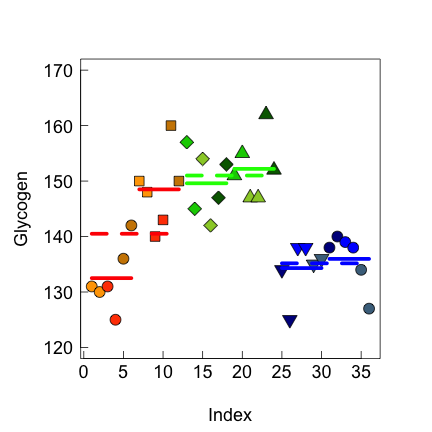
\includegraphics[width=\textwidth]{lectures/day_7_diagnostics_of_mems/figures/unnamed-chunk-3-1.png}
            \textbf{Different groupings and different variance components}
        \end{column}
    \end{columns}
\end{frame}

\begin{frame}
    \frametitle{}
    \huge\color{purple}\textbf{2. Check the Variance Components}
    \vspace{0.5cm}
    
    \normalsize\color{black}\textbf{
    A high correlation or singular fit may indicate an issue with model specification.}
\end{frame}

\begin{frame}[fragile]
    \frametitle{}
    \textbf{A correlation of exactly 1 and a singular fit?}
    \tiny
    \begin{VerbatimIN}
m.f <- lmer(root ~ week * fertilizer + (week|plant), fertilizer)
summary(m.f) 
    \end{VerbatimIN}
    \begin{VerbatimOUT}
Linear mixed model fit by REML ['lmerMod']
Formula: root ~ week * fertilizer + (week | plant)
   Data: fertilizer

REML criterion at convergence: 104.3
Scaled residuals: 
    Min      1Q  Median      3Q     Max 
-1.6916 -0.7407 -0.1264  0.6904  2.2746 
Random effects:
 Groups   Name        Variance  Std.Dev. Corr
 plant    (Intercept) 0.0306727 0.17514      
          week        0.0007169 0.02677  1.00
 Residual             0.2171683 0.46601      
Number of obs: 60, groups:  plant, 12
Fixed effects:
                       Estimate Std. Error t value
(Intercept)            -0.22233    0.21196  -1.049
week                    0.98333    0.03201  30.724
fertilizercontrol      -0.75767    0.29975  -2.528
week:fertilizercontrol -0.09167    0.04526  -2.025
Correlation of Fixed Effects:
            (Intr) week   frtlzr
week        -0.685              
frtlzrcntrl -0.707  0.484       
wk:frtlzrcn  0.484 -0.707 -0.685
optimizer (nloptwrap) convergence code: 0 (OK)
boundary (singular) fit: see ?isSingular        
    \end{VerbatimOUT}
\end{frame}

\begin{frame}[fragile]
    \frametitle{}
    \tiny
    \begin{VerbatimIN}
m.f.no <- lmer(root ~ week * fertilizer + (week||plant), fertilizer)
summary(m.f.no)         
    \end{VerbatimIN}
    \begin{VerbatimOUT}
Linear mixed model fit by REML ['lmerMod']
Formula: root ~ week * fertilizer + ((1 | plant) + (0 + week | plant))
   Data: fertilizer

REML criterion at convergence: 105
Scaled residuals: 
    Min      1Q  Median      3Q     Max 
-1.6953 -0.6984 -0.1626  0.6948  2.2986 
Random effects:
 Groups   Name        Variance Std.Dev.
 plant    (Intercept) 0.054570 0.23360 
 plant.1  week        0.001283 0.03582 
 Residual             0.218527 0.46747 
Number of obs: 60, groups:  plant, 12
Fixed effects:
                       Estimate Std. Error t value
(Intercept)            -0.22233    0.22172  -1.003
week                    0.98333    0.03353  29.325
fertilizercontrol      -0.75767    0.31355  -2.416
week:fertilizercontrol -0.09167    0.04742  -1.933
Correlation of Fixed Effects:
            (Intr) week   frtlzr
week        -0.735              
frtlzrcntrl -0.707  0.520       
wk:frtlzrcn  0.520 -0.707 -0.735
    \end{VerbatimOUT}
    \normalsize
    \textbf{Of course that is not “keeping it maximal”, but as maximal as possible}
\end{frame}

\begin{frame}
    \frametitle{}
    \huge\color{purple}\textbf{3. Check Normality of Random Effects}
    \vspace{0.5cm}
    
    \normalsize\color{black}\textbf{Use visual tools such as histograms and QQ plots to check for normality.}
\end{frame}

\begin{frame}[fragile]
    \frametitle{}
    \textbf{We use the model without correlation}
    \scriptsize
    \begin{VerbatimIN}
m.f.2 <- lmer(root ~ week * fertilizer + (week||plant), fertilizer)
VarCorr(m.f.2)            
    \end{VerbatimIN}
    \begin{VerbatimOUT}
 Groups   Name        Std.Dev.
 plant    (Intercept) 0.23360 
 plant.1  week        0.03582 
 Residual             0.46747         
    \end{VerbatimOUT}
\end{frame}

\begin{frame}[fragile]
    \frametitle{Random Intercept Check}
    \begin{columns}
        \begin{column}{0.45\textwidth}
            \textbf{Plotting}
            \scriptsize
            \begin{VerbatimIN}
hist(ranef(m.f.2)$plant[,1])                
            \end{VerbatimIN}
            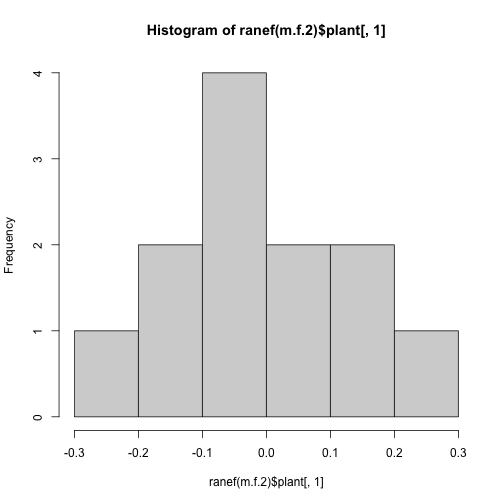
\includegraphics[width=\textwidth]{lectures/day_7_diagnostics_of_mems/figures/unnamed-chunk-14-1.png}
        \end{column}
        \begin{column}{0.55\textwidth}
            \textbf{Testing}
            \scriptsize
            \begin{VerbatimIN}
shapiro.test(ranef(m.f.2)$plant[,1])              
            \end{VerbatimIN}
            \begin{VerbatimOUT}
    Shapiro-Wilk normality test

data:  ranef(m.f.2)$plant[, 1]
W = 0.98228, p-value = 0.9912
            \end{VerbatimOUT}
        \normalsize
        \textbf{
        The Shapiro-Wilk test tests for a significant difference of the data distribution to normality, i.e. if $\mathit{p}<0.05$, the data are not normal.}
        \end{column}
    \end{columns}
\end{frame}

\begin{frame}[fragile]
    \frametitle{Random Slope Check}
    \begin{columns}
        \begin{column}{0.45\textwidth}
            \textbf{Plotting}
            \scriptsize
            \begin{VerbatimIN}
hist(ranef(m.f.2)$plant[,2])                
            \end{VerbatimIN}
            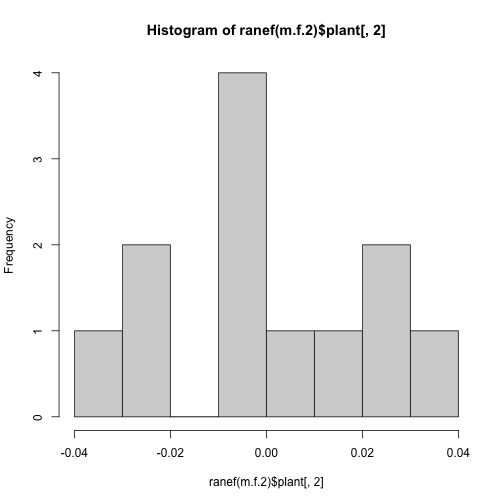
\includegraphics[width=\textwidth]{lectures/day_7_diagnostics_of_mems/figures/unnamed-chunk-16-1.png}
        \end{column}
        \begin{column}{0.55\textwidth}
            \textbf{Testing}
            \scriptsize
            \begin{VerbatimIN}
shapiro.test(ranef(m.f.2)$plant[,2])                
            \end{VerbatimIN}
            \begin{VerbatimOUT}
    Shapiro-Wilk normality test

data:  ranef(m.f.2)$plant[, 2]
W = 0.95601, p-value = 0.7257                
            \end{VerbatimOUT}
        \end{column}
    \end{columns}
\end{frame}

\begin{frame}[fragile]
\frametitle{Another useful perspective: QQ-Plots}
    \begin{columns}
        \begin{column}{0.55\textwidth}
        \textbf{Intercept ranefs}
        \scriptsize
        \begin{VerbatimIN}
qqmath(ranef(m.f.2)$plant[,1], 
panel = function(x,...) {
          panel.qqmathline(x,...)
          panel.qqmath(x,...)})                    
        \end{VerbatimIN}
            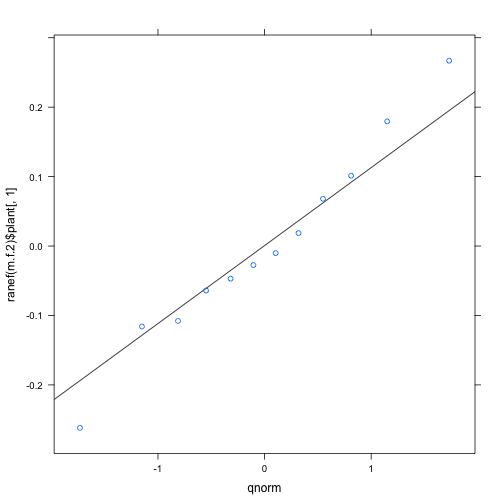
\includegraphics[width=\textwidth]{lectures/day_7_diagnostics_of_mems/figures/unnamed-chunk-18-1.png}
        \end{column}
        \begin{column}{0.55\textwidth}
        \textbf{Slope ranefs}
        \scriptsize
        \begin{VerbatimIN}
qqmath(ranef(m.f.2)$plant[,2], 
panel = function(x,...) {
          panel.qqmathline(x,...)
          panel.qqmath(x,...)})                  
        \end{VerbatimIN}
            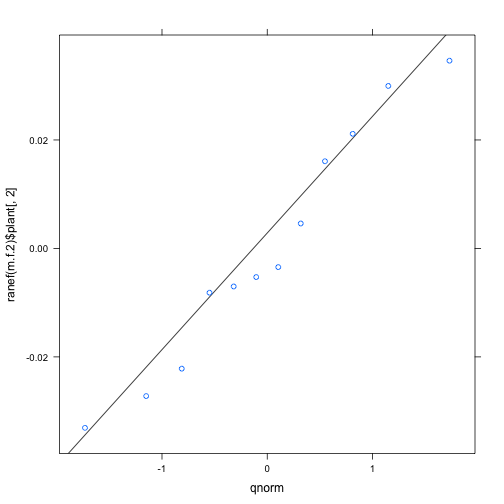
\includegraphics[width=\textwidth]{lectures/day_7_diagnostics_of_mems/figures/unnamed-chunk-19-1.png}
        \end{column}
    \end{columns}
\end{frame}


\begin{frame}[fragile]
    \frametitle{}
    \large\textbf{Note:}\\
    Too few levels of the Random Effects can make these checks difficult.
    \color{violet} e.g. with only 5 genotypes, a distribution is difficult to test.
\end{frame}

\begin{frame}[fragile]
    \frametitle{Random Effects Model: Genotype Deviations}
    \begin{columns}
        \begin{column}{0.55\textwidth}
        \scriptsize
        \begin{VerbatimIN}
m.g <- lmer(Height ~ poly(P,2) + 
(poly(P,2)|Genotype), geno)
xyplot(Height ~ P|Genotype,geno)            
        \end{VerbatimIN}
            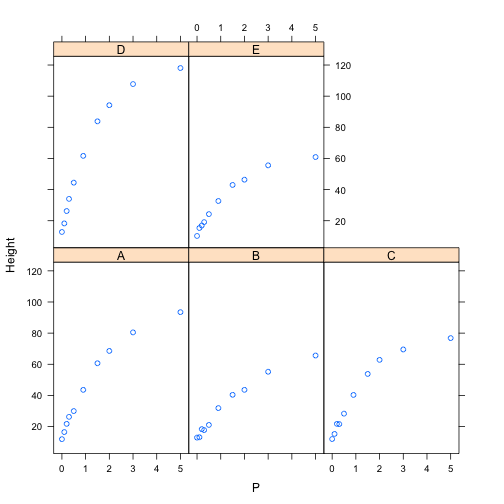
\includegraphics[width=\textwidth]{lectures/day_7_diagnostics_of_mems/figures/unnamed-chunk-21-1.png}
        \end{column}
        \begin{column}{0.55\textwidth}
        \scriptsize
        \begin{VerbatimIN}
VarCorr(m.g)                   
        \end{VerbatimIN}
        \tiny
        \begin{VerbatimOUT}
 Groups   Name        Std.Dev. Corr         
 Genotype (Intercept) 11.544                
          poly(P, 2)1 50.835    0.997       
          poly(P, 2)2 26.338   -0.989 -0.974
 Residual              2.455      
        \end{VerbatimOUT}
        \vspace{0.1cm}

        \scriptsize
        \textit{Side Note: see the complex "random slope" here}\\
        \vspace{0.5cm}
        
        \normalsize
        \textbf{Genotype-specific deciations from the non-linear population trend}
        \end{column}
    \end{columns}
\end{frame}

\begin{frame}[fragile]
    \frametitle{Distribution of Random Effects}
    \scriptsize
    \begin{VerbatimIN}
hist(ranef(m.g)$Genotype[,1])           
    \end{VerbatimIN}
    \begin{center}
    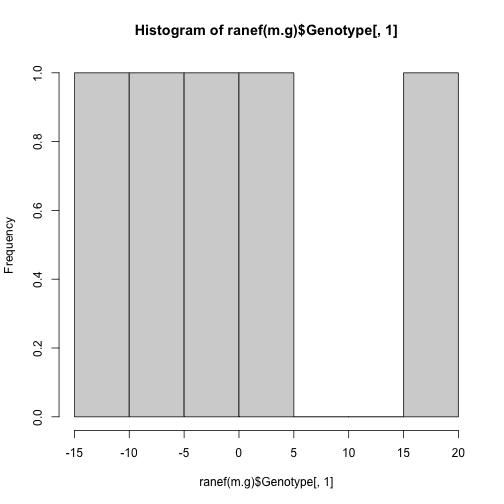
\includegraphics[width=0.65\textwidth]{lectures/day_7_diagnostics_of_mems/figures/unnamed-chunk-23-1.png}        
    \end{center}
\end{frame}

\begin{frame}
    \frametitle{}
    \huge\color{purple}\textbf{4. Check your residuals}
    \vspace{0.5cm}
    
    \normalsize\color{black}\textbf{Revisiting the Orthodont dataset for residual checks.}
\end{frame}

\begin{frame}[fragile]
    \frametitle{Plotting Residuals: Orthodont Data}
    \textbf{Use the in-built plot function for residual plots}
    \scriptsize
    \begin{VerbatimIN}
fm1 <- lmer(distance ~ age * Sex + (age|Subject))
plot(fm1)          
    \end{VerbatimIN}
    \begin{columns}
        \begin{column}{0.5\textwidth}
            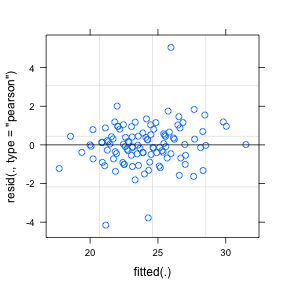
\includegraphics[width=\textwidth]{lectures/day_7_diagnostics_of_mems/figures/unnamed-chunk-25-1.png}
        \end{column}
        \begin{column}{0.5\textwidth}
        \normalsize
            You are looking at all residuals across all fitted values across all predictors and Random Effect levels. There is no strong trend visible.\\
            \textbf{But}, don't jump to conclusions just yet...
        \end{column}
    \end{columns}
\end{frame}

\begin{frame}[fragile]
    \frametitle{QQ Plot of Residuals}
    \scriptsize
    \begin{VerbatimIN}
require("lattice")
qqmath(fm1, id=0.05) # set significance level for outlier test        
    \end{VerbatimIN}
    \begin{columns}
        \begin{column}{0.5\textwidth}
            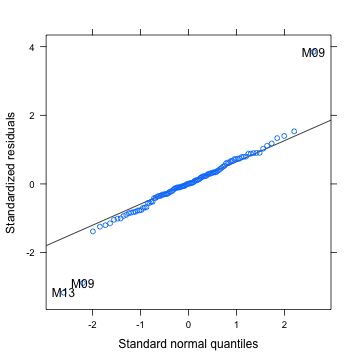
\includegraphics[width=\textwidth]{lectures/day_7_diagnostics_of_mems/figures/unnamed-chunk-26-1.png}  
        \end{column}
        \begin{column}{0.5\textwidth}
        \normalsize
            Here, we look at all residuals across all values and levels of the predictors combined. Three data points seem to deviate quite a bit.
        \end{column}
    \end{columns}
\end{frame}

\begin{frame}
    \frametitle{Residual Plotting Strategy}
    \large
    An overall plot, like the default plots produced above may...
    \vspace{0.2cm}
    
    \begin{itemize}
        \item ... mask any issues
        \item ... show issues, but don't give inside to their origin
    \end{itemize}
    \vspace{0.5cm}
    
    \textbf{Therefore: Subset the residuals in meaningful ways}
\end{frame}

\begin{frame}[fragile]
    \frametitle{Standardized Residuals vs Age}
    \scriptsize
    \begin{VerbatimIN}
fm1 <- lmer(distance ~ age * Sex + (age|Subject))
plot(fm1, resid(., scaled=TRUE) ~ age, abline = 0)        
    \end{VerbatimIN}
    \begin{columns}
        \begin{column}{0.5\textwidth}
            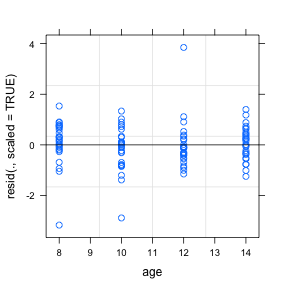
\includegraphics[width=\textwidth]{lectures/day_7_diagnostics_of_mems/figures/unnamed-chunk-27-1.png}
        \end{column}
        \begin{column}{0.5\textwidth}
        \normalsize
            Now you looks at all residuals across all values and levels of the predictor age but NOT sub-setted by Sex or Subject. Possibly some larger variance at ages 8, 10, 12?
        \end{column}
    \end{columns}
\end{frame}

\begin{frame}[fragile]
    \frametitle{Response Residuals vs Fitted Values by Age}
    \scriptsize
    \begin{VerbatimIN}
plot(fm1, resid(.) ~ fitted(.) | Sex, abline = 0)        
    \end{VerbatimIN}
    \begin{columns}
        \begin{column}{0.5\textwidth}
            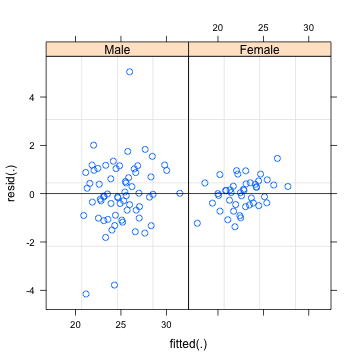
\includegraphics[width=\textwidth]{lectures/day_7_diagnostics_of_mems/figures/unnamed-chunk-29-1.png}
        \end{column}
        \begin{column}{0.5\textwidth}
        \normalsize
            AHA! Here, the spread in residuals is quite a bit larger for boys than for girls: this violates the assumption of homogeneous (constant) variance along a predictor.
        \end{column}
    \end{columns}
\end{frame}

\begin{frame}[fragile]
    \frametitle{Modeling Heterogeneous Residual Variance}
    We could try to model different residual variances for boys and girls (working with the R-side matrix).\\
    e.g. quite easily done with the 'weights' argument in nlme().
    \vspace{0.5cm}

    \scriptsize
    \begin{VerbatimIN}
mod <- lme(distance ~ age * Sex, random = ~ age|Subject, 
           weights = varIdent(form = ~1|Sex))
getVarCov(mod, type = "random.effects")
    \end{VerbatimIN}
    \begin{VerbatimOUT}
Random effects variance covariance matrix
            (Intercept)       age
(Intercept)     3.89140 -0.155210
age            -0.15521  0.024498
  Standard Deviations: 1.9727 0.15652         
    \end{VerbatimOUT}
\end{frame}

\begin{frame}[fragile]
    \frametitle{Extracting Conditional Variance-Covariance Matrix}
    \scriptsize
    \begin{VerbatimIN}
getVarCov(mod, individuals = 1, type = "conditional")            
    \end{VerbatimIN}
    \tiny
    \begin{VerbatimOUT}
Subject M01 
Conditional variance covariance matrix
       1      2      3      4
1 2.6555 0.0000 0.0000 0.0000
2 0.0000 2.6555 0.0000 0.0000
3 0.0000 0.0000 2.6555 0.0000
4 0.0000 0.0000 0.0000 2.6555
  Standard Deviations: 1.6296 1.6296 1.6296 1.6296         
    \end{VerbatimOUT}
    \scriptsize
    \begin{VerbatimIN}
getVarCov(mod, individuals = 27, type = "conditional") 
    \end{VerbatimIN}
    \tiny
    \begin{VerbatimOUT}
Subject F11 
Conditional variance covariance matrix
        1       2       3       4
1 0.44389 0.00000 0.00000 0.00000
2 0.00000 0.44389 0.00000 0.00000
3 0.00000 0.00000 0.44389 0.00000
4 0.00000 0.00000 0.00000 0.44389
  Standard Deviations: 0.66625 0.66625 0.66625 0.66625         
    \end{VerbatimOUT}
\end{frame}

\begin{frame}[fragile]
    \frametitle{}
    \scriptsize
    \begin{VerbatimIN}
mod        
    \end{VerbatimIN}
    \tiny
    \begin{VerbatimOUT}
Linear mixed-effects model fit by REML
  Data: NULL 
  Log-restricted-likelihood: -205.7612
  Fixed: distance ~ age * Sex 
  (Intercept)           age     SexFemale age:SexFemale 
   16.3406250     0.7843750     1.0321023    -0.3048295 
Random effects:
 Formula: ~age | Subject
 Structure: General positive-definite, 
            Log-Cholesky parametrization
            StdDev    Corr  
(Intercept) 1.9726633 (Intr)
age         0.1565175 -0.503
Residual    1.6295843       
Variance function:
 Structure: Different standard deviations per stratum
 Formula: ~1 | Sex 
 Parameter estimates:
     Male    Female 
1.0000000 0.4088466 
Number of Observations: 108
Number of Groups: 27 
    \end{VerbatimOUT}
    \scriptsize
    \begin{VerbatimIN}
mod$sigma^2*0.4088466^2        
    \end{VerbatimIN}
    \tiny
    \begin{VerbatimOUT}
[1] 0.443889
    \end{VerbatimOUT}
\end{frame}

\begin{frame}[fragile]
    \frametitle{Modeling among-group variances}
    We could also try to model different \textbf{among-group} variances for boys and girls (working with the G-side matrix).
    \vspace{0.3cm}

    \scriptsize
    \begin{VerbatimIN}
model <- lme(distance ~ age * Sex,
random = list(Subject = pdDiag(form = ~ Sex),
              Subject = pdSymm(form = ~ age)))        
    \end{VerbatimIN}
    \vspace{0.5cm}

    \normalsize
    \textit{pdDiag}: diagonal positive-definite matrix \\
    \textit{pdSymm}: general positive-definite matrix
\end{frame}

\begin{frame}[fragile]
    \frametitle{Extracting among-group variances}
    \scriptsize
    \begin{VerbatimIN}
VarCorr(mod)
    \end{VerbatimIN}
    \begin{VerbatimOUT}
Subject = pdLogChol(age) 
            Variance   StdDev    Corr  
(Intercept) 3.89140059 1.9726633 (Intr)
age         0.02449773 0.1565175 -0.503
Residual    2.65554484 1.6295843     
    \end{VerbatimOUT}
    \begin{VerbatimIN}
VarCorr(model)        
    \end{VerbatimIN}
    \begin{VerbatimOUT}
            Variance    StdDev    Corr  
Subject =   pdDiag(Sex)                 
(Intercept) 1.60666457  1.2675427       
SexFemale   0.89043771  0.9436301       
Subject =   pdSymm(age)                 
(Intercept) 4.09538269  2.0237052 (Intr)
age         0.03252448  0.1803454 -0.829
Residual    1.71620369  1.3100396              
    \end{VerbatimOUT}
\end{frame}



\begin{frame}[fragile]
    \frametitle{}
    \huge\color{purple}\textbf{5. Check your residuals on the random effects level}
    \vspace{0.5cm}
    
    \normalsize\color{black}\textbf{}
\end{frame}

\begin{frame}[fragile]
    \frametitle{Standardized residuals by Subject}
    \scriptsize
    \begin{VerbatimIN}
plot(fm1, Subject ~ resid(.))        
    \end{VerbatimIN}
    \begin{columns}
        \begin{column}{0.5\textwidth}
            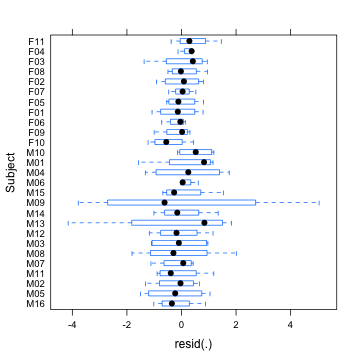
\includegraphics[width=\textwidth]{lectures/day_7_diagnostics_of_mems/figures/unnamed-chunk-36-1.png}
        \end{column}
        \begin{column}{0.5\textwidth}
        \normalsize
            Both M09 and M13 (two boys) have much larger variances than any of the other children, which is in line with the finding that boys have a larger residual variance than girls in their growth.
        \end{column}
    \end{columns}
\end{frame}

\begin{frame}[fragile]
    \frametitle{Observed versus fitted values by Subject}
    \scriptsize
    \begin{VerbatimIN}
plot(fm1, distance ~ fitted(.) | Subject, abline = c(0,1))        
    \end{VerbatimIN}
    \begin{columns}
        \begin{column}{0.6\textwidth}
            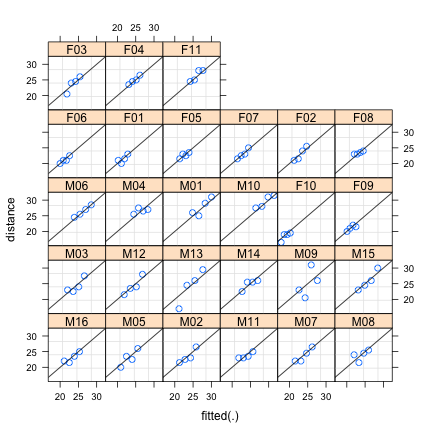
\includegraphics[width=\textwidth]{lectures/day_7_diagnostics_of_mems/figures/unnamed-chunk-37-1.png}
        \end{column}
        \begin{column}{0.4\textwidth}
        \normalsize
            Again we see that M09 and M13 have much larger variances than any of the other children.
        \end{column}
    \end{columns}
\end{frame}

\begin{frame}[fragile]
    \frametitle{Standardized residuals along age, separated by Subject}
    \scriptsize
    \begin{VerbatimIN}
plot(fm1, resid(.) ~ age | Subject, abline = 0)        
    \end{VerbatimIN}
    \begin{columns}
        \begin{column}{0.6\textwidth}
            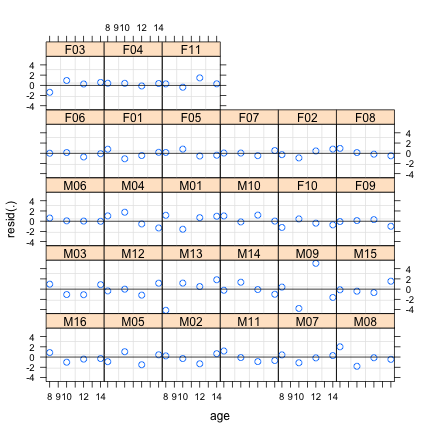
\includegraphics[width=\textwidth]{lectures/day_7_diagnostics_of_mems/figures/unnamed-chunk-38-1.png}
        \end{column}
        \begin{column}{0.4\textwidth}
        \normalsize
            Again observe the spread in M09 and M13 (in the latter, it is one data point)
        \end{column}
    \end{columns}
\end{frame}

\begin{frame}
    \frametitle{Modeling Within-Group Variance}
    \large
    We could now model the within-group/residual variance better by allowing each child its own variance (in contrast to the standard in LMEMs to assume the same variance within each level of a grouping variable)
    \vspace{0.5cm}
    
    \textit{More on Heterogeneuos Variance models using nlme():} \color{blue}\href{https://quantdev.ssri.psu.edu/sites/qdev/files/ILD_Ch06_2017_MLMwithHeterogeneousVariance.html}{here}
\end{frame}

\begin{frame}[fragile]
    \huge\color{purple}\textbf{Convergence issue checks with lme4}
\end{frame}

\begin{frame}[fragile]
    \frametitle{1. Check for Singularity: True}
    \scriptsize
    \begin{VerbatimIN}
VarCorr(m.f)        
    \end{VerbatimIN}
    \tiny
    \begin{VerbatimOUT}
 Groups   Name        Std.Dev. Corr 
 plant    (Intercept) 0.175136      
          week        0.026774 1.000
 Residual             0.466013            
    \end{VerbatimOUT}
    \scriptsize
    \begin{VerbatimIN}
isSingular(m.f)        
    \end{VerbatimIN}
        \tiny
    \begin{VerbatimOUT}
[1] TRUE        
    \end{VerbatimOUT}
    \scriptsize
    \begin{VerbatimIN}
VarCorr(m.f.2)        
    \end{VerbatimIN}
        \tiny
    \begin{VerbatimOUT}
 Groups   Name        Std.Dev.
 plant    (Intercept) 0.23360 
 plant.1  week        0.03582 
 Residual             0.46747         
    \end{VerbatimOUT}
    \scriptsize
    \begin{VerbatimIN}
isSingular(m.f.2)
    \end{VerbatimIN}
    \begin{VerbatimOUT}
[1] FALSE
    \end{VerbatimOUT}
\end{frame}

\begin{frame}[fragile]
    \frametitle{2. Action: Scale Predictors}
    \begin{equation*}
        scale(\mathbf{x}) = \frac{\mathbf{x} - mean(\mathbf{x})}{sd(\mathbf{x})}
    \end{equation*}
    \vspace{0.3cm}
    
    \scriptsize
    \begin{Verbatim}[numbers=left,numbersep=6pt,frame=single]
m.f.scaled <- 
lmer(root ~ scale(week) * fertilizer + (scale(week)|plant), fertilizer)
VarCorr(m.f.scaled) 
    \end{Verbatim}
    \begin{Verbatim}[numbers=left,numbersep=6pt,frame=single]
 Groups   Name        Std.Dev. Corr 
 plant    (Intercept) 0.335781      
          scale(week) 0.076364 1.000
 Residual             0.466013
    \end{Verbatim}

    \begin{Verbatim}[numbers=left,numbersep=6pt,frame=single]
isSingular(m.f.scaled)
---
[1] TRUE
    \end{Verbatim}
    \normalsize That did not help...
\end{frame}

\begin{frame}[fragile]
    \frametitle{3. Specify Starting Values for Parameters}
    \scriptsize
    \begin{Verbatim}[numbers=left,numbersep=6pt,frame=single]
a <- getME(m.f,c("theta")) # re-param estimates
b <- getME(m.f,c("beta")) # fixed param estimates

m.check <- lmer(root ~ week * fertilizer + (week|plant), 
            data = fertilizer,
            start=list(theta=a,fixef=b))

isSingular(m.check)
    \end{Verbatim}
    \begin{Verbatim}[numbers=left,numbersep=6pt,frame=single]
[1] TRUE
    \end{Verbatim}
     \normalsize That did not help either...
    
\end{frame}

\begin{frame}[fragile]
    \frametitle{4. Compare Potential Optimizers}
    \scriptsize
    \begin{Verbatim}[numbers=left,numbersep=6pt,frame=single]
modelfit.all <- lme4::allFit(m.f)    
    \end{Verbatim}
    \begin{Verbatim}[numbers=left,numbersep=6pt,frame=single]
bobyqa : [OK]
Nelder_Mead : [OK]
nlminbwrap : [OK]
nmkbw : [OK]
optimx.L-BFGS-B : [OK]
nloptwrap.NLOPT_LN_NELDERMEAD : [OK]
nloptwrap.NLOPT_LN_BOBYQA : [OK]        
    \end{Verbatim}
\end{frame}

\begin{frame}[fragile]
    \frametitle{Fixed effects are very similar across optimizers}
    \scriptsize
    \begin{Verbatim}[numbers=left,numbersep=6pt,frame=single]
ss <- summary(modelfit.all)
ss$fixef 
    \end{Verbatim}
    \begin{Verbatim}[numbers=left,numbersep=6pt,frame=single]
                              (Intercept)      week fertilizercontrol
bobyqa                         -0.2223333 0.9833333        -0.7576667
Nelder_Mead                    -0.2223333 0.9833333        -0.7576667
nlminbwrap                     -0.2223333 0.9833333        -0.7576667
nmkbw                          -0.2223333 0.9833333        -0.7576667
optimx.L-BFGS-B                -0.2223333 0.9833333        -0.7576667
nloptwrap.NLOPT_LN_NELDERMEAD  -0.2223333 0.9833333        -0.7576667
nloptwrap.NLOPT_LN_BOBYQA      -0.2223333 0.9833333        -0.7576667
                              week:fertilizercontrol
bobyqa                                   -0.09166667
Nelder_Mead                              -0.09166667
nlminbwrap                               -0.09166667
nmkbw                                    -0.09166667
optimx.L-BFGS-B                          -0.09166667
nloptwrap.NLOPT_LN_NELDERMEAD            -0.09166667
nloptwrap.NLOPT_LN_BOBYQA                -0.09166667
    \end{Verbatim}
\end{frame}

\begin{frame}[fragile]
    \frametitle{Residual checks using Simulations}
    \begin{itemize}
        \item[Step 1:] Simulate responses under the postulated model you want to test
        \item[Step 2:] Do that many, many times
        \item[Step 3:] Create a distribution of these simulated residuals
        \item[Step 4:] Compare new residuals against observed residuals to check whether they are atypical
    \end{itemize}
    \vspace{0.3cm}

    \textit{If the model is correctly specified, simulated and observed values should be similar}
\end{frame}

\begin{frame}[fragile]
    \frametitle{Residual Simulations with DHARMa}
    Residual simulations are implemented in the package DHARMa by Florian Hartig
    \begin{Verbatim}
library(DHARMa)        
    \end{Verbatim}
    \vspace{0.3cm}
    
    \begin{itemize}
        \item The DHARMa package documentation can be found in the vignette to the package: \href{https://cran.r-project.org/web/packages/DHARMa/vignettes/DHARMa.html}{here}.
    \end{itemize}
    \vspace{0.3cm}
    
    More on DHARMa later this week, as it is not necessary for Linear Mixed Effects Models, but helpful for GLMMs
\end{frame}

\begin{frame}
    \frametitle{Recap of Day 7}
    \textbf{After today you should know and understand}
    \begin{itemize}
        \item How a \textbf{Linear Mixed Effects Model} can be diagnosed by checking the \textbf{variance components} (no variance should be exactly zero, no correlation should be exactly -1 or 1)
        \item Checking the normal distribution of the \textbf{Random Effects}
        \item Plotting \textbf{residuals}, also for the unique RE levels (subsetting)
        \item Possible solutions: more complex R-side and G-side matrices (NOT expected for this course !)
    \end{itemize}
    \vspace{0.3cm}
    \textbf{Todays exercises on diagnosing LMEMs}
\end{frame}

\end{document}